% Motivation: explosion of exposure-employment papers + our contribution.
% (The METR-capability frame has been moved to 06_results_diffindiff.tex,
% just before the agentic re-anchor.)

\begin{frame}{AI and the future of work: in the headlines}
\centering
\begin{tikzpicture}
  \useasboundingbox (-6.5, -2.7) rectangle (6.5, 2.7);
  \node<1->[rotate=-4] at (-4, 0) {%
    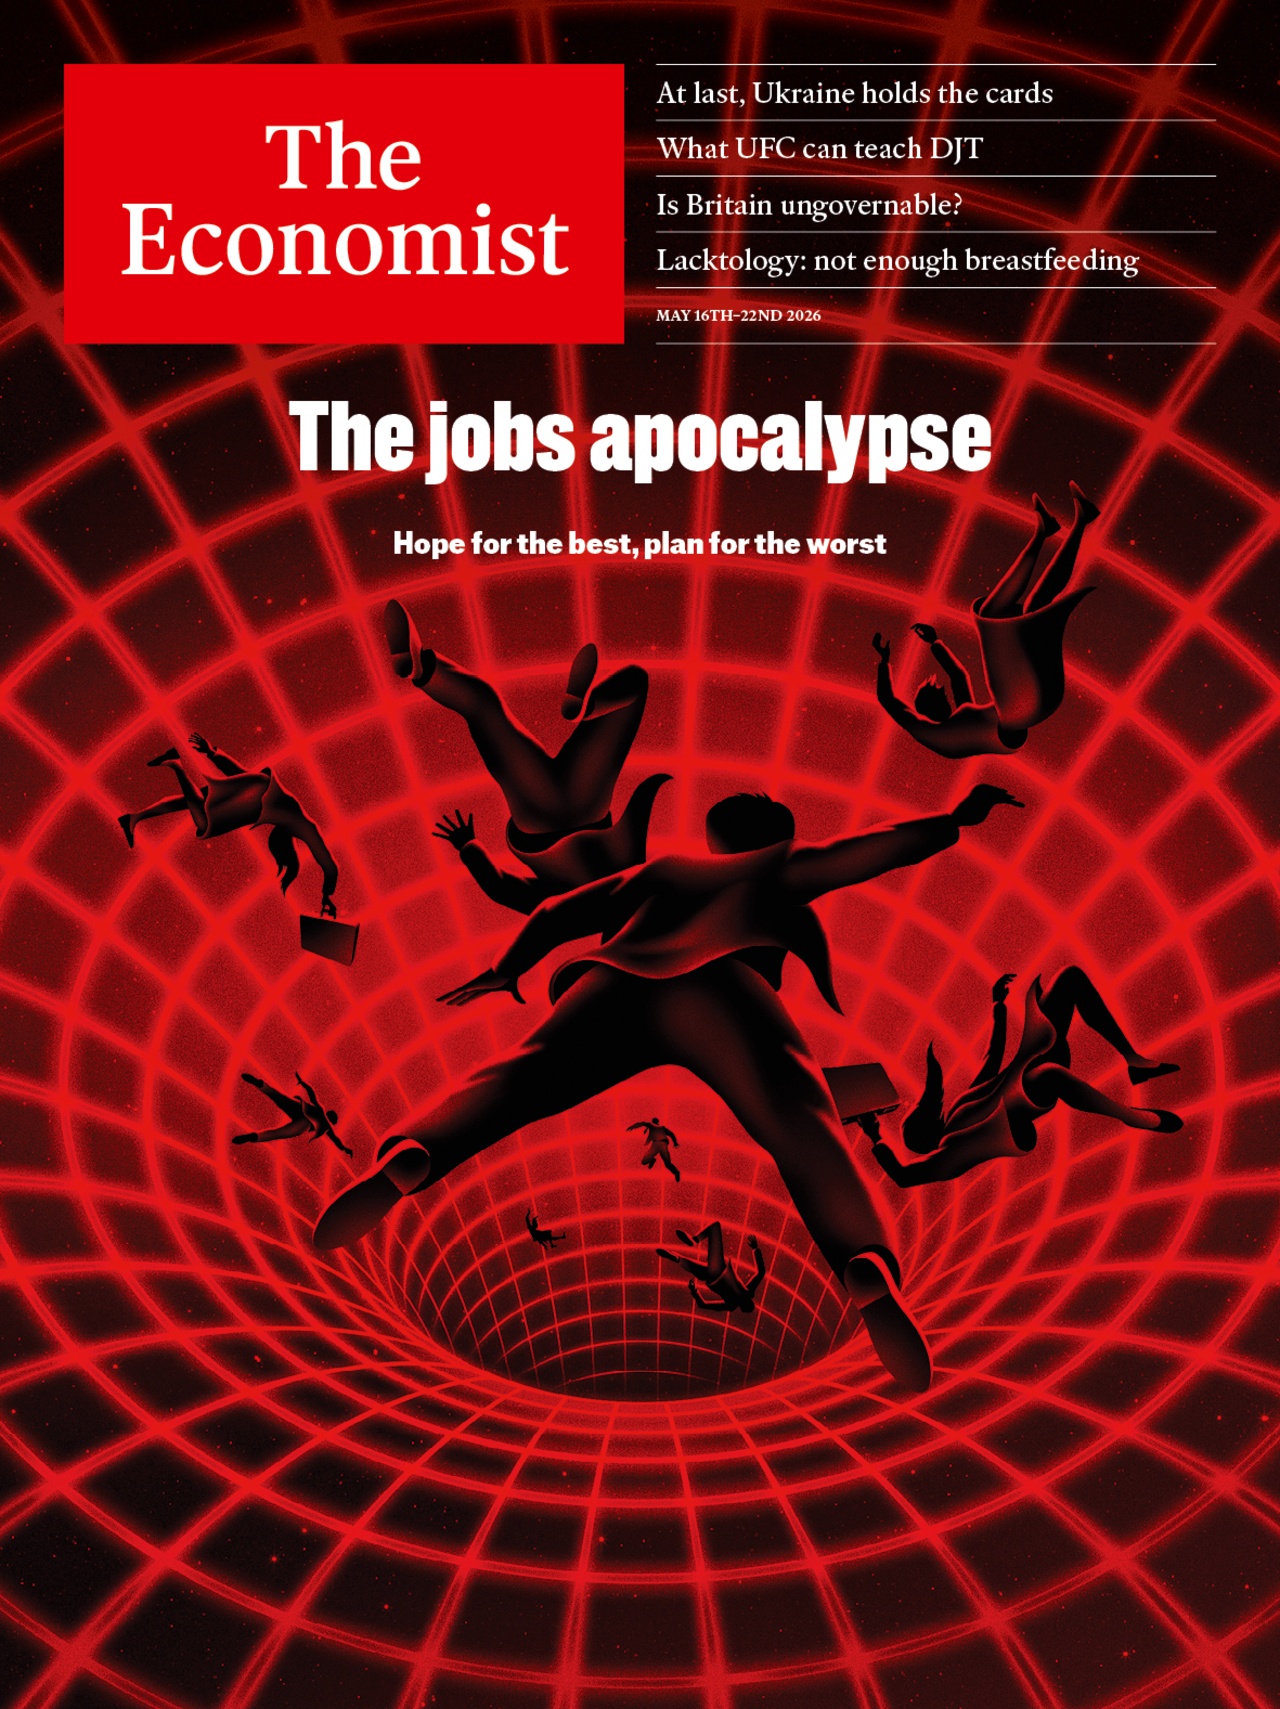
\includegraphics[height=5cm,keepaspectratio]{Economist_jobs_apocalypse.jpg}};
  \node<2->[rotate=3]  at (0, -0.3) {%
    \includegraphics[height=5cm,keepaspectratio]{{Atlantic_AI Has Ruined the Job Market}.JPG}};
  \node<3->[rotate=-2] at (4, 0.2) {%
    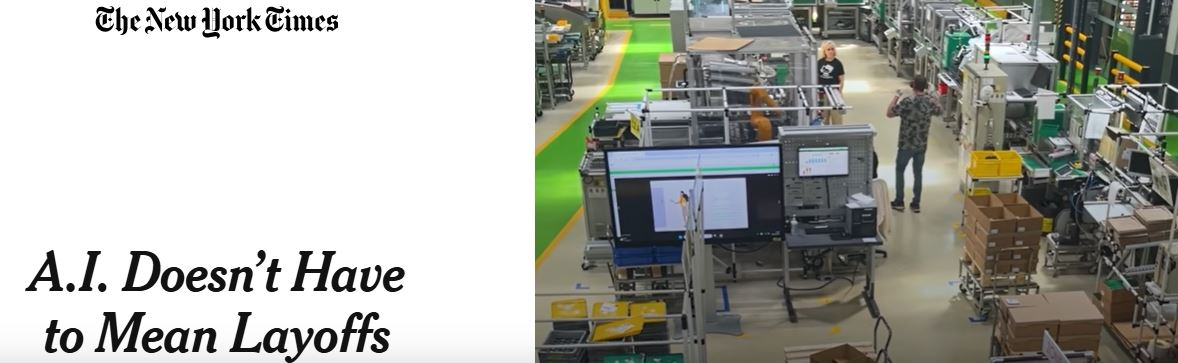
\includegraphics[height=5cm,keepaspectratio]{NYTimes_AIdoesnthavetomeanlayoffs.JPG}};
\end{tikzpicture}

\vspace{0.4em}
\end{frame}

% ---------------------------------------------------------------
\begin{frame}{Recent literature: AI exposure and employment}
\footnotesize
\setlength{\tabcolsep}{4pt}
\begin{tabular}{l l p{6.8cm}}
\toprule
Country & Paper & Headline (youngest workers, top quintile) \\
\midrule
United States  & Brynjolfsson, Chandar \& Chen (2025) & Q5 ages 22--25 decline $\sim 16$ log pts \\
Sweden         & Lodefalk et al.\ (2026)              & Q5 ages 22--25 decline $\sim 5.5\,\%$; monotonic gradient \\
United Kingdom & Teeselink (2025)                     & $-0.3\%$ per SD LLM (large language model) exposure; concentrated in junior, high-wage \\
39 countries   & Teeselink (2026)                     & Hiring declines; sharper under strict employment protection legislation \\
Denmark        & Humlum \& Vestergaard (2026)         & Null at firm level: workplace adoption rules out effects $> 1/3$ ppt on early-career share \\
Finland        & Kauhanen et al.\ (2024, 2025, 2026)  & Null; demographic explanation \\
\bottomrule
\end{tabular}

\vspace{0.8em}
\end{frame}

% ---------------------------------------------------------------
\begin{frame}{Contributions}
\begin{itemize}\setlength{\itemsep}{8pt}
  \item Complement the international literature on AI exposure and employment pre/post ChatGPT with results on Norway  
  \item Study the recent impact of \textbf{Agentic AI} ( \emph{``autonomous LLM-based systems that plan, use tools, and execute multi-step research tasks''} (Korinek, 2025)) 
  \item Track developments of the universe of Norwegian employment ``live'' 
\end{itemize}
\end{frame}
